\chapter{Introduction to Photonics}
\minitoc
\textit{All material in this chapter was created using the notes of Dr. D. Graham.}
\pagebreak

\section{Measurement of light's power}

There are two main ways of quantifying an electromagnetic waves power: radiometric and photometric.
Photometric is how much power will be seen by the human eye, while radiometric is a direct measurement of the waves power.
In these cases, light is defined as being in the visible spectrum although radiometry covers ultraviolet and infrared radiation.
The photometric measurement uses a standard responsivity of the human eye which is defined by the $V(\lambda)$ curve shown in figure \ref{fig:ItP:eye}.
\begin{figure}[H]
	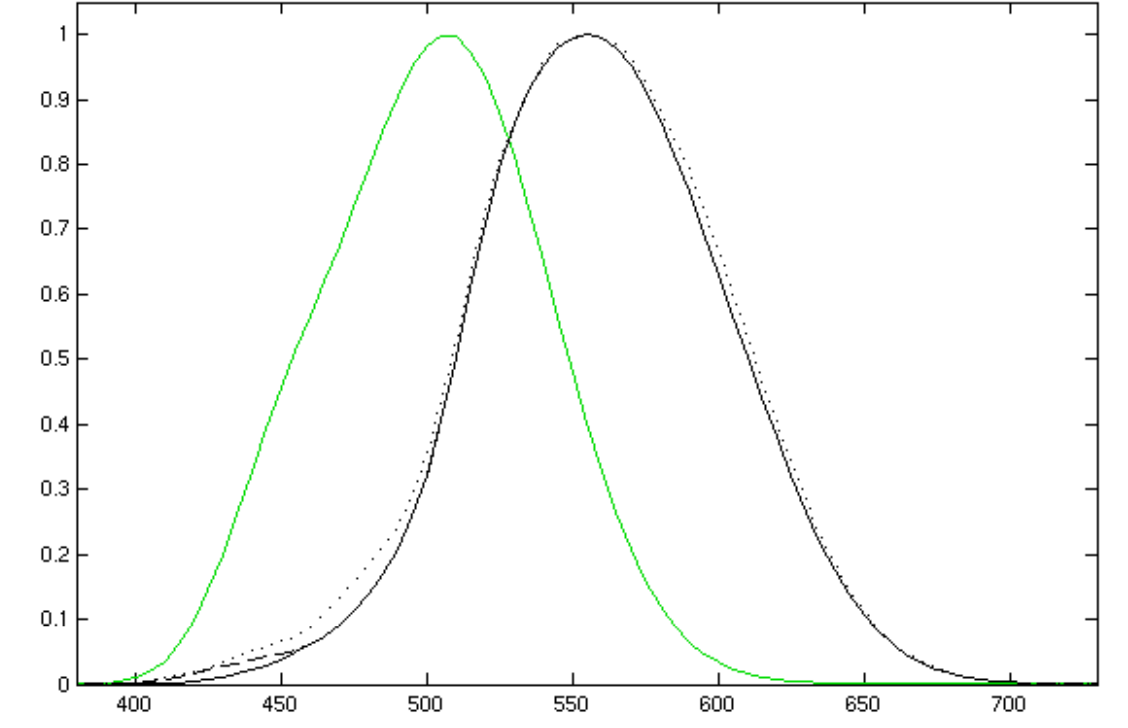
\includegraphics[width=\linewidth]{Photonics/eye}
	\caption{The graph shows the curve for the photopic response, the black line, and the scotopic response, the green line, of a standard human eye}
	\label{fig:ItP:eye}
\end{figure}
%
There are two main types of responses: the scotopic (the green line) for an eye adapted to the dark, and the photopic (the black line) for an eye adapted to bright light.
 The radiant flux spectral distribution, $\phi_e(\lambda)$, can be used to calculate the (photometric) luminous flux, $\phi_v$ using
%
\begin{equation}
	\phi_v = K\int{V(\lambda)\phi_e(\lambda)d\lambda},
	\label{eq:ItP:luminous}
\end{equation}
%
where $K$ is the spectral luminous efficiency defined as $683$ lmW$^{-1}$.
\section{Polarisation}

For the most part the basics of polarisation are the same as in \textit{Wave Optics} although the definition of circularly polarised light may be different.
 For example, right hand circularly polarised light is defined as when you look towards the source with light coming towards you, you can curl your right hand in the direction of the rotation with the thumb pointing towards you. %This is terrible, I'm sorry
 The same applies for left hand circularly polarised light, although with the left hand.
 S- and p-polarised light mean the same thing as they do in \textit{Wave Optics}.
 \\
 \begin{figure}[H]
 	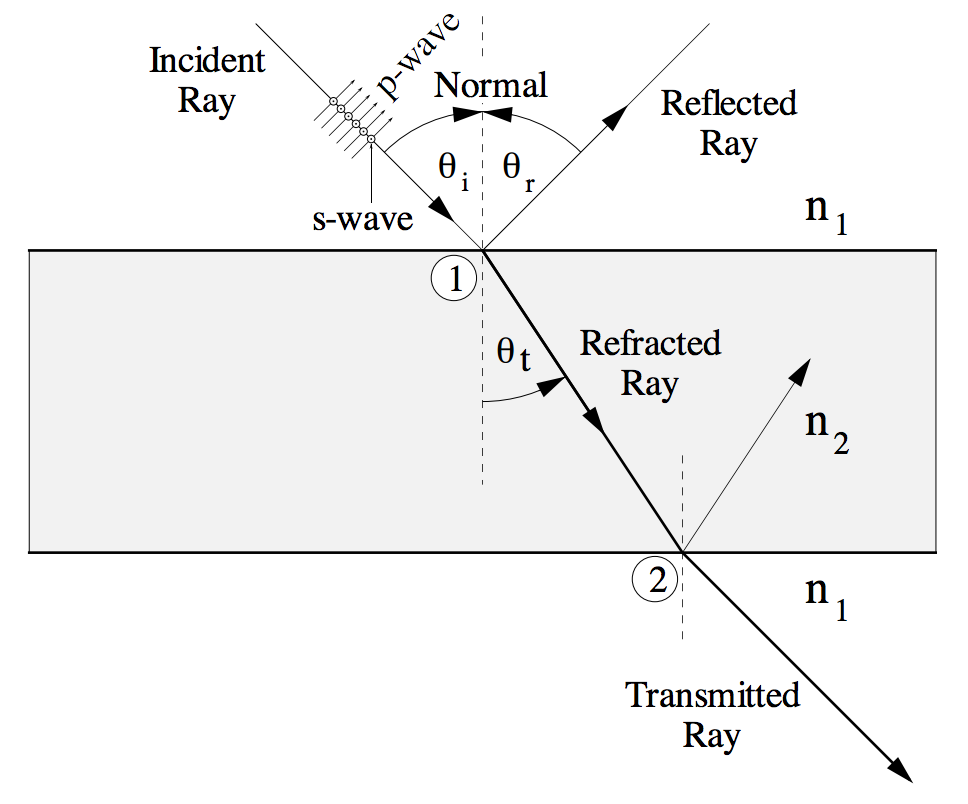
\includegraphics[width=15pt,scale=0.6]{Photonics/pho_polarisation_1}
 	
 	\label{fig:ItP:polarisation1}
 \end{figure}
 The intensity reflection coefficient, $R$, for incident light, $\theta_i$ = 0, is
 \begin{equation}
 R = \left(\frac{n_1-n_2}{n_1+n_2}\right)^2,
 \end{equation}
 where \(n_1\) and \(n_2\) are the respective refractive indices of the materials as seen in figure \ref{fig:ItP:polarisation1}. 
 For light that isnt incident at \(\theta = 0\), there is an equation for the coeffiecient of reflection for both s- and p-polarised light:
 \begin{equation}
 R_s = \left(\frac{\sin(\theta_i - \theta_t)}{\sin(\theta_i + \theta_t)}\right)^2
 \end{equation}
 \begin{equation}
R_p  = \left(\frac{\tan(\theta_i - \theta_t)}{\tan(\theta_i + \theta_t)}\right)^2.
 \end{equation}
A beam can be made to be p-polarised by passing it through multiple glass plates as the s-polarised light will be reflected much more and after multiple plates will be effectively gone.
\subsection{Birefringence}
\begin{minipage}{0.47\linewidth}
	\begin{figure} [H]
		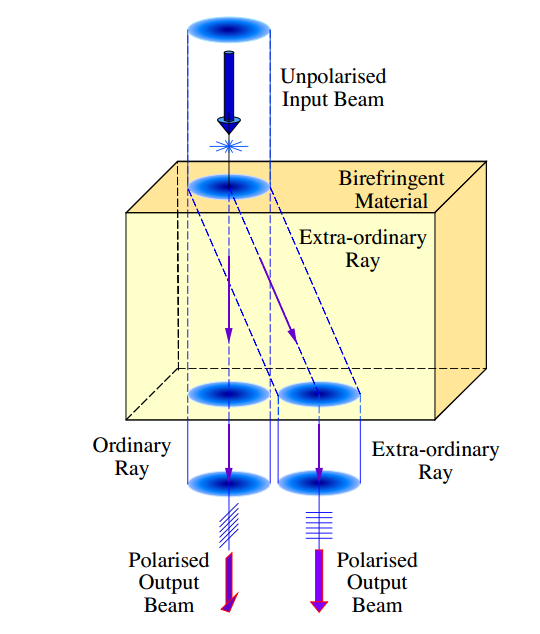
\includegraphics[width=\linewidth,scale=0.7]{Photonics/birefr_eg}
		\label{fig:ItP:birefr_1}
		%Issue with size, will get back to later
	\end{figure}	
\end{minipage}
\begin{minipage}{0.47\linewidth}
	Some materials have a special property which causes them to be birefringent. 
	 In this course, only uniaxial birefringence will be considered and this is where there are two refractive indices for the different polarisations. 
	 The birefringence gives rise to two different waves: ordinary rays (o-rays) and extraordinary rays (e-rays) \footnote{As a side note: the e-ray does not follow Snell's Law.}.
	 As the refractive indices for the waves aren't the same, they are refracted at different angles causing separation and possibly two rays to exit the material, as shown in figure \ref{fig:ItP:birefr_1}.
	As can be seen in the figure, the beams are orthogonally polarised.
\end{minipage}

A useful way of visualising  the difference between the e and o-ray is by considering the Huygens wavelets of each ray. 
\\
\begin{minipage}{0.4\linewidth}
	\begin{figure}[H]
		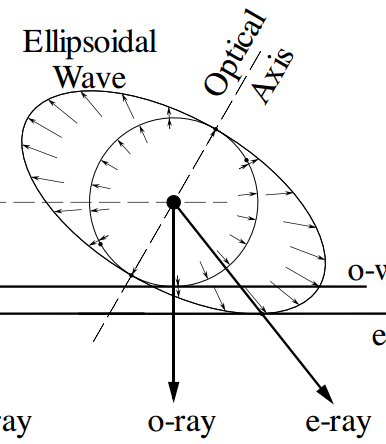
\includegraphics[,width=150pt]{Photonics/erayhuygens}
		\label{fig:ItP:bire_eray}
		
	%Yes I will make my own version of this, I'm just lazy atm even thought it is simple.
	\end{figure}
\end{minipage}
\begin{minipage}{0.6\linewidth}
	These wavelets will have a radius based on their speed in a particular direction which is polarisation dependent. 
	For the o-ray the wavelet would be circular in shape as \(n_o\) is constant in all directions while the e-ray has a more ellipical wavelet due to the non constant refractive index \(n_e\).
	The diagonal line going through the centre in figure \ref{fig:ItP:bire_eray} is the Optical Axis (OA) and is the direction in which both waves have the same refractive index.
\end{minipage}
The velocity of the e-ray along a direction is given by
\begin{equation}
	v_{e-ray} = \frac{v_ev_o}{\sqrt{v_o^2\sin[2](\theta)+v_e^2\cos[2](\theta)}}.
	\label{eq:ItP:v_e-ray}
\end{equation}
\(v_e\) and \(v_o\) are the velocities of the rays in the direction that gives the largest radius of their respective wavelets.
\(\theta\) is the angle between the OA and the e-ray.
\subsubsection{Glan-Taylor beamsplitter}
\begin{minipage}{0.47\linewidth}
	\begin{figure}[H]
	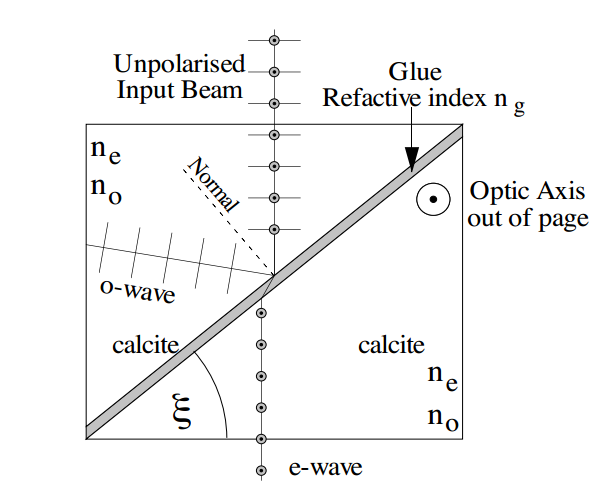
\includegraphics[scale=0.7]{Photonics/beamsplitter}
	\end{figure}
\end{minipage}
\begin{minipage}{0.47\linewidth}
	The Glan-Taylor beamsplitter is one of the more common forms of beamsplitters and often made of two pieces of calcite with a glue interface seperating them.  
	The OA is chosen so that it is perpendicular to the incoming light beam. 
	This causes the e and o-rays to travel together until they reach the glue at which the two rays diverge. 
	The o-ray is reflected while the e-ray refracts through the glue due to the differing refractive indices of the two rays.
	The second calcite crystal is included to realign the beam after the glue.
\end{minipage}
\subsubsection{Retardation plate}
This is fairly similar to the beamsplitter although in this case there is no glue interface.
The o- and e-rays therefore travel in the same direction through the beam, assuming the initial beam enters at \(90\deg\) to the face of the plate. 
As they have differring refractive indices the rays will travel at different speeds creating a phase difference between the two.
This phase difference, \(\Delta\phi\), is given by 
\begin{equation}
\Delta\phi = \frac{2\pi}{\lambda}\left(n_e - n_o\right)d
\label{eq:ItP:phase_difference}
\end{equation}
where d is the length of the birefringent material which the rays travel through.
This phase difference is where its name 'retardation plate' comes from.
\\
There are two special cases which will be considered in this course for the retardation plate: the quarter wave plate and the half wave plate.
The half wave plate will be discussed later in the course.
In the quarter wave plate case, 
\begin{align*}
\Delta\phi &= \abs{\frac{\pi}{2}} \\
 \therefore \Delta{nd} &=\abs{\frac{\lambda}{4}} 
\end{align*}
where \(\Delta{n} = n_e-n_o\).
If we recall from the form of circularly polarised light, we can see that the quarter wave plate transforms linearly polarised light into circular and vice versa. 
This requires that the incident light is at an angle of \(45\deg\) to the OA. 
Conventionally, the retardation direction is called the \emph{slow} axis, and the phase advancement direction the \emph{fast} axis.
 
\subsection{Jones matrices and vectors}
To assist in the calculation of polarisation states we will introduce Jones matrices and vectors. 
\\
It is important to note that these only work with fully polarised light.
\\
\subsubsection{Beams of light}
Using an example polarised beam,
\begin{align*}
\vb{E}(z,t) &= E_x(z,t)\vb{i} + E-y(z,t)\vb{j}\\
		&= e^{i(\omega{t} - kz)}\left[E_{0x}e^{i\phi_x} + E_{0y}e^{i\phi_y}\right]\\
		&= \mqty[E_{0x}e^{i\phi_x} \\ E_{0y}e^{i\phi_y}]e^{i(\omega{t} -kz)} .
\end{align*}
The first term at the end is called the unnormalised Jones vector and the second term is a common factor to all polarisations so can be ignored.
\\
A simple polarisation state is along the x-axis, e.g. \(\theta = 0\), can be represented as 
\[\vb{E}_0 = E_{0x}e^{i\phi_x}\mqty[1 \\ 0]\]
which has no y-axis dependancy.
It is vital to realise that the angle of polarisation is measured counter clockwise from the x-axis.
\\
Commonly, however, the normalised versions are used:
\begin{align*}
\vb{E}_0 &= \mqty[1 \\ 0]\\
\vb{E}_{90} &= \mqty[0 \\ 1]\\
\vb{E}_{45} &= \frac{1}{\sqrt{2}}\mqty[1 \\ 1]\\
\vb{E}_{135} &= \frac{1}{\sqrt{2}}\mqty[1 \\ -1]\\
\vb{E}_{RHC} &= \frac{1}{\sqrt{2}}\mqty[1 \\ -i]\\
\vb{E}_{LHC} &= \frac{1}{\sqrt{2}}\mqty[1 \\ i]\\.
\end{align*}
\subsubsection{Polarizers and wave plates}
Polarizers and waveplates are represented by Jones matrices and normal matrix multiplication rules can be used to calculate the resulting polarisation state of light after passing through one or more.
The general formula for the Jones matrix of a polarizer, polarised at an angle \(\theta\) to the x-axis, is:
\begin{equation}
A_J^{L\theta} = \mqty[\cos[2](\theta) & \sin(\theta)\cos(\theta) \\ \sin(\theta)\cos(\theta) & \sin[2](\theta)].
\label{eqn:ItP:Polarizermat}
\end{equation}
The general Jones matrices for the quarter wave plates with horizontal and vertical fast axes are:
\begin{align}
A_J^{QH} &= e^{i\frac{\pi}{4}}\mqty[1 & 0 \\ 0 & i]  \label{eqn:ItP:QHmat} \\
A_J^{QV} &= e^{i\frac{\pi}{4}}\mqty[1 & 0 \\ 0 & -i]. \label{eqn:ItP:QVmat}
\end{align}
The matrix for a half wave plate is:
\begin{align}
A_J^{H\theta} = \mqty[\cos 2\theta & \sin 2\theta \\ \sin 2\theta & -\cos 2\theta].
\label{eqn:ItP:HwpMat}
\end{align}
\\
When multiplying Jones matrices, the order is important.
The left most matrix will be the matrix representing the last wave plate or polarizer that the beam of light passes through. 
The right most matrix will likewise be the first that the light passes through.
The Jones vector representing the beam of light will be the on the right of the last matrix.
\subsection{Stokes parameters}
These were introduced in *hesitantly guesses* \textit{Electromagnetism} in the form:
\begin{align*}
S_0 &= \abs{\vb{E}_x}^2 + \abs{\vb{E}_y}^2 = E_{0x}^2 + E_{0y}^2 \\
S_1 &= \abs{\vb{E}_x}^2 - \abs{\vb{E}_y}^2 =  E_{0x}^2 - E_{0y}^2 \\
S_2 &= 2\Re{\vb{E}_x\vb{E}_y^*} = 2E_{0x}E_{0y}\cos{\epsilon} \\
S_3 &= 2\Im{\vb{E}_x\vb{E}_y^*} = 2E_{0x}E_{0y}\sin{\epsilon}
\end{align*}
where \(\epsilon\) is a potentially time variant phase as seen from the general wave equation:
\begin{equation*}
\vb{E}(z,t) = \Re{E_{0x}\vb{i}e^{i(\omega{t} - kz)} + E_{0y}\vb{j}e^{i(\omega{t} - kz + \epsilon)}}.
\end{equation*}
\\
These can be normalised by dividing by \(S_0\) to get:
\begin{align*}
P_1 &= \frac{E_{0x}^2 - E_{0y}^2}{E_{0x}^2 + E_{0y}^2} \\
P_2 &= \frac{2E_{0x}E_{0y}\cos{\epsilon}}{E_{0x}^2 + E_{0y}^2} \\
P_3 &= \frac{2E_{0x}E_{0y}\sin{\epsilon}}{E_{0x}^2 + E_{0y}^2}.
\end{align*}
The degree of polarisation, \(P_{tot}\) is therefore defined as
\[P_{tot}^2 = P_{1}^2 + P_{2}^2 + P_{3}^2\] 
\[ 0 \leq P_{tot}^2 \leq 1\]
where 0 is unpolarised and 1 is fully polarised.
